São funçõees do tipo: $\mathbb{R}^3\longrightarrow \mathbb{R}$\\

Superfícies de nível são um conjunto de pontos no espaço tridimensional
onde uma função de três variáveis atinge um valor constante. 
Elas são obtidas ao igualar a função a uma constante, como $(w=k)$.
Essa visualização tridimensional é análoga às curvas de nível usadas em 
mapas topográficos para representar a altitude.\\
\medskip                
\begin{figure}[H]
\centering
\includegraphics[width=0.6\linewidth]{Fig17.png}
\caption{Hiperbóide Circular}
\end{figure}

\begin{enumerate}
  \item Equação do Plano: \[ z= ax+by+c \]
  \[\Big\{(x,y,z)\in Dom. f; f(x,y,z)=c\Big\}\]
  \item Parabolóide Eliptico. Para a e b > 0.
  \[ z=ax^2+by^2 \]
  \item Parabolóide hiperbólico. 
  \[ z=ax^2-by^2 \]
  \item Cilindros.
      \begin{enumerate}
    \item Cilindro Parabólico. Cada corte $z=c$ é uma parábola.
      \[ z=x^2 \]
    \item Cilindro Eliptico. \[ x^2+y^2=1 \]
      \end{enumerate}
  \item Superfícies Quádricas.
      \begin{enumerate}
          \item Elipsóide.
          \[\frac{x^2}{a^2}+\frac{y^2}{b^2}+\frac{z^2}{c^2}=1\]
          \item Hiperbolóide de uma folha.
          \[\frac{x^2}{a^2}+\frac{y^2}{b^2}-\frac{z^2}{c^2}=1\]
          \item Hiperbolóide de duas folhas.
          \[-\frac{x^2}{a^2}-\frac{y^2}{b^2}+\frac{z^2}{c^2}=1\]
      \end{enumerate}
      \bigskip
      \begin{table}[H]
\centering
\caption{Superfícies quádricas usuais}
\label{tab:quadricas}
\begin{tabular}{lccc}
\toprule
\textbf{Superfície}   & \textbf{a} &\textbf{b} & \textbf{c} \\
\midrule
Elipsóide             & +          & +         & +\\
Hiperbolóide 1 Folha  & +          & +         & -\\
Hiperbolóide 2 folhas & -          & +         & -\\ 
\bottomrule
\end{tabular}
\end{table}
  \item Superfícies Esféricas.
  A esfera não é uma função de (x,y)
  \item Superfícies Compostas.
      \begin{enumerate}
        \item Cone.
        \[ z=\sqrt{x^2+y^2} \]
        \item Superfície Helicoidal.
        \[\begin{cases}
          &x=r\cos(\theta)\\
          &y=r\sen(\theta)\\
          &z=c\theta\\
        \end{cases}\]
        onde:\\
        r é o raio (distância do eixo)\\
        $\theta$ é o parâmetro angular (rad.)\\
        c é uma constante que controla o passo da hélice(quanto o ponto
        sobe em z a cada volta completa)
      \end{enumerate}
\end{enumerate}
Para funções de uma variável:
\[ y=f(x) \] temos:
\[
\lim_{x\rightarrow x_0} f(x)
\]

\begin{figure}[H]
    \centering
    \begin{tikzpicture}[>=latex, scale=1.1]
      % parâmetro para a posição de x0 (altere se quiser)
      \def\xo{0}

      % Eixo x
      \draw[-] (-4,0) -- (4,0) node[right] {$x$};

      % Marca de x0
      \draw (\xo,-0.15) -- (\xo,0.15) node[above=2pt] {$x_0$};

      % Aproximação pela esquerda: x -> x0^{-}
      \draw[->, line width=0.8pt] (-3,0.6) -- (\xo-0.2,0.6)
            node[midway, above=2pt] {$x\to x_0^{-}$};
      \node at (-1.6,0.95) {\large $-$};

      % Aproximação pela direita: x -> x0^{+}
      \draw[->, line width=0.8pt] (3,-0.6) -- (\xo+0.2,-0.6)
            node[midway, below=2pt] {$x\to x_0^{+}$};
      \node at (1.6,-0.95) {\large $+$};
    \end{tikzpicture}
    \caption{$\displaystyle \lim_{x\to x_0} f(x)$}
\end{figure}
Para funções de duas variáveis temos que:
\[z=f(x,y)\]\qquad\[\lim_{(x_0\rightarrow(x_0,y_0))}f(x,y)\]
\[l=\lim_{(x,y)\rightarrow(x_0,y_0)}\]
Próximo de l, o quanto desejarmos, desde que seja tomado $(x,y)$ 
o suficiente próximo de $(x_0, y_0)$.\\
\begin{figure}[H]
    \centering
    % Requer: \usepackage{pgfplots}  % (pgfplots já carrega o tikz)
    % \pgfplotsset{compat=1.18}
\begin{tikzpicture}[>=latex, scale=1.1]
  % --- parâmetros do ponto ---
  \def\xo{1.8}
  \def\yo{1.2}
  \def\arr{0.7} % comprimento das setas

  % eixos
  \draw[->] (-0.5,0) -- (4,0) node[right] {$x$};
  \draw[->] (0,-0.5) -- (0,3) node[above] {$y$};

  % ponto (x0,y0)
  \filldraw (\xo,\yo) circle (1.5pt) node[above right] {$(x_0,y_0)$};

  % projeções tracejadas nos eixos
  \draw[dashed] (\xo,0) -- (\xo,\yo) node[pos=0,below] {$x_0$};
  \draw[dashed] (0,\yo) -- (\xo,\yo) node[pos=0,left] {$y_0$};

  % --- 4 setas apontando para (x0,y0) ---
  % em x (da esquerda e da direita)
  \draw[->,thick,shorten >=2pt] (\xo-\arr,\yo) -- (\xo,\yo);
  \draw[->,thick,shorten >=2pt] (\xo+\arr,\yo) -- (\xo,\yo);

  % em y (de baixo e de cima)
  \draw[->,thick,shorten >=2pt] (\xo,\yo-\arr) -- (\xo,\yo);
  \draw[->,thick,shorten >=2pt] (\xo,\yo+\arr) -- (\xo,\yo);
    % setas diagonais a 45° (sentido anti-horário)
  \draw[->,thick,shorten >=2pt] ({\xo+\arr/sqrt(2)},{\yo-\arr/sqrt(2)}) -- (\xo,\yo);
  \draw[->,thick,shorten >=2pt] ({\xo-\arr/sqrt(2)},{\yo+\arr/sqrt(2)}) -- (\xo,\yo);


  % (opcionais) rótulos das setas:
  % \node at (\xo-\arr/2,\yo+0.15) {$\Delta x$};
  % \node at (\xo+\arr/2,\yo+0.15) {$\Delta x$};
  % \node at (\xo+0.15,\yo-\arr/2) {$\Delta y$};
  % \node at (\xo+0.15,\yo+\arr/2) {$\Delta y$};
\end{tikzpicture}
\caption{Ponto $(x_0, y_0)$ em $f(x,y)$ com setas em $x$ e $y$.}
\end{figure}

\textbf{Exemplo.}
\medskip
\[f(x,y,x)\to (x^2+y^2+z^2).
\text{Domínio: } D(f)=\mathbb{R}^3
\quad\text{e}\quad
\text{Imagem: } I(f)=(0,\infty)
\]

%%\textbf{Superfícies de nível.}

\[x^2+y^2+z^2=c\]

Se $c>0$: a função é de uma esfera de centro $(0,0,0,)$ e raio c.\\
Se $c=0\Longrightarrow I=(0,0,0)$\\
Se $c<0 \Longrightarrow \nexists$ a superfície de nível.

%\subsubsection{\textbf{Exemplo.}}
\[z^2=3(x^2+y^2)=0\]
Dividindo toda a equação por 3 temos:
\[\frac{z^3}{3}=x^2+y^2=0\]\,
$\therefore$\[\frac{z^2}{3}-x^2-y^2=0\]
Isso é um cone circular duplo.
\begin{figure}[H]
    \centering
    \includegraphics[width=.8\linewidth]{Fig15.png}
    \caption{Cone circular duplo}
\end{figure}

Se c=1, 

\[\frac{z^3}{3}=x^2+y^2=1\]\,
$\therefore$\[\frac{z^2}{3}-x^2-y^2=1\]

Isso é um hiperbolóide de duas folhas.

Se c=-1 o gráfico será o de um paraboloide de uma folha.
\begin{figure}[H]
    \centering
    \includegraphics[width=.6 \linewidth]{fig14.jpg}
    \caption{Hiperbóide de uma folha.}
\end{figure}
% \usepackage{booktabs} no preâmbulo
\begin{table}[H]
\centering
\caption{Superfícies quádricas usuais}
\begin{tabular}{ll}
\toprule
\textbf{Nome} & \textbf{Equação (forma padrão)} \\
\midrule
Elipsóide              & $\dfrac{x^2}{a^2}+\dfrac{y^2}{b^2}+\dfrac{z^2}{c^2}=1$ \\
Hiperbolóide de 1 folha& $\dfrac{x^2}{a^2}+\dfrac{y^2}{b^2}-\dfrac{z^2}{c^2}=1$ \\
Hiperbolóide de 2 folhas& $-\dfrac{x^2}{a^2}-\dfrac{y^2}{b^2}+\dfrac{z^2}{c^2}=1$ \\
Cone elíptico          & $\dfrac{x^2}{a^2}+\dfrac{y^2}{b^2}-\dfrac{z^2}{c^2}=0$ \\
Parabolóide elíptico   & $\dfrac{x^2}{a^2}+\dfrac{y^2}{b^2}=\dfrac{z}{c}$ \\
Parabolóide hiperbólico& $\dfrac{x^2}{a^2}-\dfrac{y^2}{b^2}=\dfrac{z}{c}$ \\
Cilindro elíptico      & $\dfrac{x^2}{a^2}+\dfrac{y^2}{b^2}=1$ \\
Cilindro hiperbólico   & $\dfrac{x^2}{a^2}-\dfrac{y^2}{b^2}=1$ \\
\bottomrule
\end{tabular}
\end{table}

A Tabela \ref{tab:quadricas} traz o nome da quádrica e a sua equação.
\subsection{Limites de funções de duas variáveis.}



\[\lim_{(x,y)\to(x_0,y_0)}=l\] se $|f(x,y)|-l=0$

$\lim_{(x,y)}\to (x,y)$ independente do caminho.
\[ \partial\qquad d(x,y) \]
\textbf{Observação.} Sejae $f(x,y)\rightarrow l_1,$, se $(x,y)
\rightarrow
(x_0,y_0)$ sobre um caminho $c_1$, então podemos afirmar que
 o $lim f(x,y)$ não existe. $(x,y)\rightarrow(x_0,y_0)$.

\textbf{Exemplo 1.}
\[\lim_{(x,y)\rightarrow(1,2)}(\frac{x^2+y^2}{x})=\frac{1+4}{1}=5\]

\textbf{Exemplo 2.}
\[\lim_{(x,y)\rightarrow(1,-1)}\frac{\ln(xy^2)}{x^2+y^2+1}
=\frac{\ln 1}{1+1+1}=\frac{0}{3}=0\]

\textbf{Exemplo 3.}
\[\lim_{(x,y)\rightarrow(0,0)}\frac{1}{x^2+y^2}=\frac{1}{0}=\infty\]

\textbf{Exemplo 4.}
\[\lim_{(x,y)\to(0,0)}\frac{\sin(xy)}{xy}\]
Pela identidade Trigonométrica temos:
\[\sin(a+b)=\sin(a)\cos(b)+\sin(b)\cos(a)\]
e,
\[\sin(2a)=\sin(2a)\cos(2a)+\sin(2a)\cos(2a)=\]
\[2\sin(2a)\cos(2a) \]

e pelo limite fundamental,
\[\lim_{(x,y)\rightarrow(0,0)}\frac{\sin(\theta)}{\theta}=1\]
Podemos dizer que,

\[\lim_{(x,y)\rightarrow(0,0)}\frac{\sin(xy)}{xy}=1\]
\begin{figure}[H]
    \centering
    \includegraphics[width=.6 \linewidth]{fig16.png.png}
    \caption{$\lim_{(x,y)\rightarrow(0,0)}\frac{\sin(\theta)}{\theta}=1$}
\end{figure}

\textbf{Exemplo 5.}
\[\lim_{(x,y)\rightarrow(0,0)}\frac{x^2}{x^2+y^2}\]
Primeiramente fixamos x em zero e variamos y.
\[\lim_{(x,y)\rightarrow(0,y)}\frac{x^2}{x^2+y^2}=\frac{0}{y^2}\]

De outra forma, podemos fixa y em zero e variamos o x.

\[\lim_{(x,y)\to(x,0)}\frac{x^2}{x^2+y^2}=\frac{x^2}{x^2}=1\]

\textbf{Exemplo 6.}

Aqui vamos primeiro fixar o y, depois fixamos o x e em seguida usamos 
o caminho de $x=y$ conforme mostra a Figura\,\ref{gráfico da reta xy}

\[\lim_{(x,o)\rightarrow(x,x)}\frac{2xy}{x^2+y^2}=\frac{x^2}{x^2}=1\]
% requer: \usepackage{pgfplots} e \pgfplotsset{compat=1.18}
\begin{figure}[H]
  \centering
  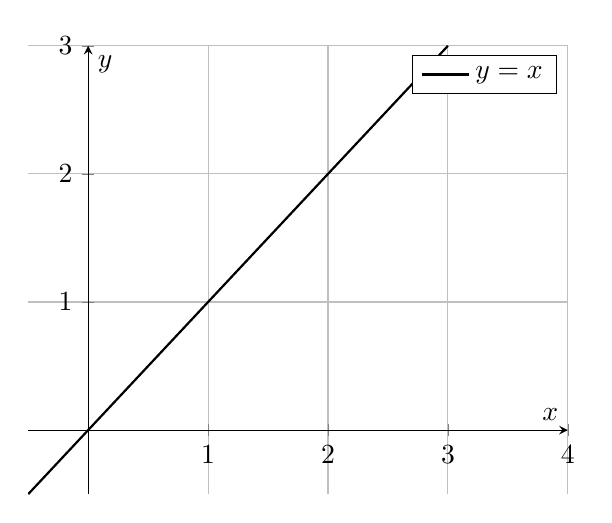
\begin{tikzpicture}
    \begin{axis}[
      axis lines=middle, xlabel={$x$}, ylabel={$y$},
      xmin=-0.5, xmax=4, ymin=-0.5, ymax=3,
      grid=both
    ]
      \addplot[domain=-0.5:3, samples=2, thick] {x};
      \addlegendentry{$y=x$}
    \end{axis}
  \end{tikzpicture}
  \caption{Reta $y=x$}
  \label{gráfico da reta xy}
\end{figure}

então,\\
\textbf{variando x}

\[\lim_{(x,y)\to(x,0)}\frac{2xy}{x^2+y^2}=\frac{0}{x^2}=0\]

\textbf{variando y}

\[\lim_{(x,y)\to(0,y)}\frac{2xy}{x^2+y^2}=\frac{0}{y^2}=0\]

\textbf{na reta $x=y$},

\[\lim_{(x,y)\rightarrow(x,x)}\frac{2x^2}{x^+x^2}=\frac{2x^2}{2x^2}=1\]
\[\therefore\qquad\lim_{(x,y)\rightarrow(x,x)}\frac{2x^2}{x^+x^2}\qquad\nexists\]
E o motivo para isso é que os limites calculados em caminhos diferentes não
são iguais.\\
\medskip
\textbf{Exemplo 7.}
\[\lim_{(x,y)\rightarrow(0,0)}\frac{x^3}{x^2+y^2}\]

\begin{enumerate}
    \item Variando x,
    \[\lim_{(x,y)\to(x,0)}\frac{x^3}{x^2+y^2}=\frac{x^3}{x^2}=x\]
    e se $x=0$
    
    \[\lim_{(x,y)\rightarrow(0,0)}\frac{x^3}{x^2+y^2}=0\]
    \item Variando y,
    \[\lim_{(x,y)\rightarrow(0,y)}\frac{x^3}{x^2+y^2}=\frac{0}{y^2}=0\]
    \item Seguindo o caminho da parábola $x^2:f(x,x^2)$
    
    \begin{figure}[H]
\centering
\begin{tikzpicture}
  \begin{axis}[
    axis lines=middle,
    xlabel={$x$}, ylabel={$y$},
    xmin=-3, xmax=3, ymin=-1, ymax=9,
    samples=200,
    domain=-3:3
  ]
    % (x, x^2) equivale a y = x^2
    \addplot[thick] {x^2};
  \end{axis}
\end{tikzpicture}
\caption{Gráfico de $(x, x^2)$, isto é, $y=x^2$.}
\end{figure}
\[\lim_{(x,y)\rightarrow(x,x^2)}\frac{x^3}{x^2+y^2}=\frac{0}{y^2}=0\]
\[\frac{x^3}{x^2+x^4}=\frac{x^3}{x^2(1+x^2)}=\frac{x}{1+x^2}\]

levando ao limite, temos:
\[\lim_{(x,y)\rightarrow(x,x^2)}\frac{x^3}{x^2+y^2}=\frac{0}{1}=0\]

\item Seguindo pelo caminho da parábola $x=y^2$
\end{enumerate}
% Requer: \usepackage{pgfplots}
% \pgfplotsset{compat=1.18}

\begin{figure}[H]
\centering
\begin{tikzpicture}
  \begin{axis}[
    axis lines=middle,
    xlabel={$x$},
    ylabel={$y$},
    xmin=-1, xmax=9,
    ymin=-3, ymax=3,
    domain=-3:3,
    samples=200,
    axis equal image
  ]
    % x = y^2  →  (x(t), y(t)) = (t^2, t)
    \addplot[very thin, no marks, parametric] ({x^2},{x});
  \end{axis}
\end{tikzpicture}
\caption{Gráfico da curva $x = y^2$ traçada como $(t^2,t)$.}
\label{fig:xy2}
\end{figure}
Aqui temos $f(y^2,y)$.
\[f(y^2,y)=\frac{y^6}{y^4+y^2}=\frac{y^{\cancel{6}4}}{\cancel{y^2}(y^2+1)}=(0,0)\]
\[|f(x,y)-0|=\frac{x^3}{x^2+y^2}\]

Se $(x,y)\to(0,0)$, então $d\big((x,y),(0,0)\big)=\sqrt{x^2+y^2}\to 0$.

Então pelo teorema do confronto,
\[\lim_{(x,y)\to(0,0)}\frac{x^3}{x^2+y^2}=\lim_{(x,y)\to(0,0)}\frac{0}{0+y^2}=0\]

\textbf{Exemplo 8.}
\begin{enumerate}
  \item \[\lim_{(x,y)\to(0,0)}\frac{x^3}{x^2+y^2}\]
\[y=0\to f(x,0)=\lim_{(x,y)\to(0,0)}\frac{x^3}{x^2+y^2}\]
  \item \[\lim_{(x,y)\to(x,0)}\frac{x^2y}{x^4+y^2}=\frac{0}{x^4}=0\]
  \item \[\lim_{(x,y)\to(0,y)}\frac{x^2y}{x^4+y^2}=\frac{0}{y^2}=0\]
  \item \[\lim_{(x,y)\to(x,x)}\frac{x^3}{2x^2}=\frac{x}{2}\]
\[ \therefore\qquad\nexists\quad\lim_{x,y\to(0,0)f(x,y0)} \]
\end{enumerate}
\newpage
\subsection{Derivadas Parciais.}
\[ z = f(x,y) \quad \text{fazendo $y$ constante} \]

A taxa de variação de $f$ em relação à variável x no ponto $(x_0,y_0)$ é 
obtida quando mantemos y constante em relação a $y_0$ e fazemos a 
derivada de f em relação a x para $x=x_0$

Definição: A derivada parcial de $f$ em relação a x no ponto 
$(x_0,y_0)$ é dada por:
\[ \lim_{h\to0}\frac{f(x_0-f_1, y)-f(x-y_0)}{h}\]

Notação:
\[ f_x(x_0,y_0),\, \frac{\partial f}{\partial x},\, f_1,\, D_x(x,y) \]

A derivada também pode ser em relação a y com x constante.

\[ \lim_{h\to0}\frac{f(x_0, y+h)-f(x_0-y)}{h}\qquad \text{se}
\lim(f)\exists\]

Notação:
\[ f_y,\,\frac{\partial f}{\partial y},\,f_y,\,D_f(x,y) \]

\subsubsection{\textbf{Exemplo.}}% primeiro exemplo de derivadas parciais.

Derivação em relação a x.
\begin{align*}
  &f(x,y)=xy^2,\,(x_0,y_0)=(-1,2)\\
  &f_x(-1,2)= \lim_{h\to0}\frac{f((-1+h),2)-f(-1,2)}{h}=\\
  &\lim_{h\to 0}\frac{(-1+h)\cdot 4-(-4)}{h}=4 
\end{align*}

Derivação a y.
\begin{align*}
  &f(x,y)=xy^2,\,(x_0,y_0)=(-1,2)\\
  &f_y(-1,2)= \lim_{h\to0}\frac{f((-1,2+h))-f(-1,2)}{h}=\\
  &\lim_{h\to 0}\frac{(-(2+h)^2)- 4-(-4)}{h}=-4 
\end{align*}
\textbf{Valem as propriedades operativas da derivada a uma variável.}
\[\begin{cases}
  &f_x=y^2\to f(-1,2)=2^2=4\\
  &f_y=2xy\to f(-1,2)=2(-1)2=-4 \\
\end{cases}\]
\subsubsection{\textbf{Exemplo.}}
\[\begin{cases}
  &f(x,y)=x^2+xy+3y-1,\quad P=f(0,1)\\
  &f_x=2x+y\to f_(0,1)=1
\end{cases}\]
\subsubsection{\textbf{Exemplo.}}
\begin{align*}
  &f(x,y)=xe^{x^2y},\qquad P(x_0,y_0)=(1,\ln2)\\
  &u=x\to u'=1\\
  &v=e^{x^2y}\to v'=e^{x^2y}\cdot2xy
\end{align*}
Usando a regra do produto $(v\cdot u)'=u'v+uv'$, então,
\[\begin{cases}
  &f_x= e^{x^2y}+xe^{x^2y}\cdot2xy\to f_x(P)=e^{\ln2}+e^{\ln2}\cdot\ln2=2+2\ln2\\
  &f_y= xe^{x^2y}\cdot2xy\to f_x(P)=e^{\ln2}\cdot2\ln2
\end{cases}\]
\subsubsection{Exemplo.}
Seja a função 
\[f(x,y)=y\sin(xy)+\frac{x^2}{y+1},\qquad\text{no ponto} P(x_0,y_0)=(3,0)\]
(derivação em relação a x)
Aqui é preciso usar a regra do produto.
\[ \begin{cases}
  &f_x=y2\cos(xy)\to f_x(3,0)+\dfrac{2x}{y+1}=\cancel{y^2\cos(xy)}
  +\dfrac{2x}{y+1}=6\\
  &f_y=\cancel{1}\cdot\sin(xy)+xy\cos(xy)-\dfrac{x^2}{(y+1)^2}\to f_y(3,0)=-9

\end{cases} \]